\documentclass[main.tex]{subfiles}

\begin{document}
\sloppy


\vspace{1.0cm}

\section{Redesign gerarchia dei FixtureComponent}\label{sec:FixtureComponentHierachy}
I FixtureComponent formano uno strato che si pone tra i dati DMX che arrivano ad UnrealEngine ed i materiali visti nel capitolo precedente. Mentre i materiali Light/Lens/Beam definiscono come effettuare il rendering della luce emessa da un faro, i FixtureComponent ne controllano i comportamenti e comunicano con i primi attraverso i parametri presenti nei vari moduli della pipeline che abbiamo creato in precedenza. Un altro modo che i FixtureComponent hanno per interagire con un faro istanziato in un mondo virtuale è andando direttamente a modificarne le proprietà come, ad esempio, la rotazione delle varie geometrie. \newline

In questo capitolo analizzeremo i problemi riscontrati nell'implementazione di un nuovo componente e proporremo una nuova gerarchia atta all'aggiunta di nuove features nella maniera più semplice possibile.

\subsection{Stato preliminare}\label{subsec:3_oldImplementation}
I FixtureComponent sono, realmente, delle classi organizzate in una struttura gerarchica. Alla base abbiamo \lstinline{FixtureComponentBase}, esteso da \lstinline{SimpleAttributeFixtureComponent} che rappresenta singole features che vengono controllate in maniera diretta e da \lstinline{MultipleAttributeFixtureComponent} che invece riguarda features che vengono controllate da più canali, oppure che possono avere comportamenti avanzati.
\begin{figure}[H]
    \centering
    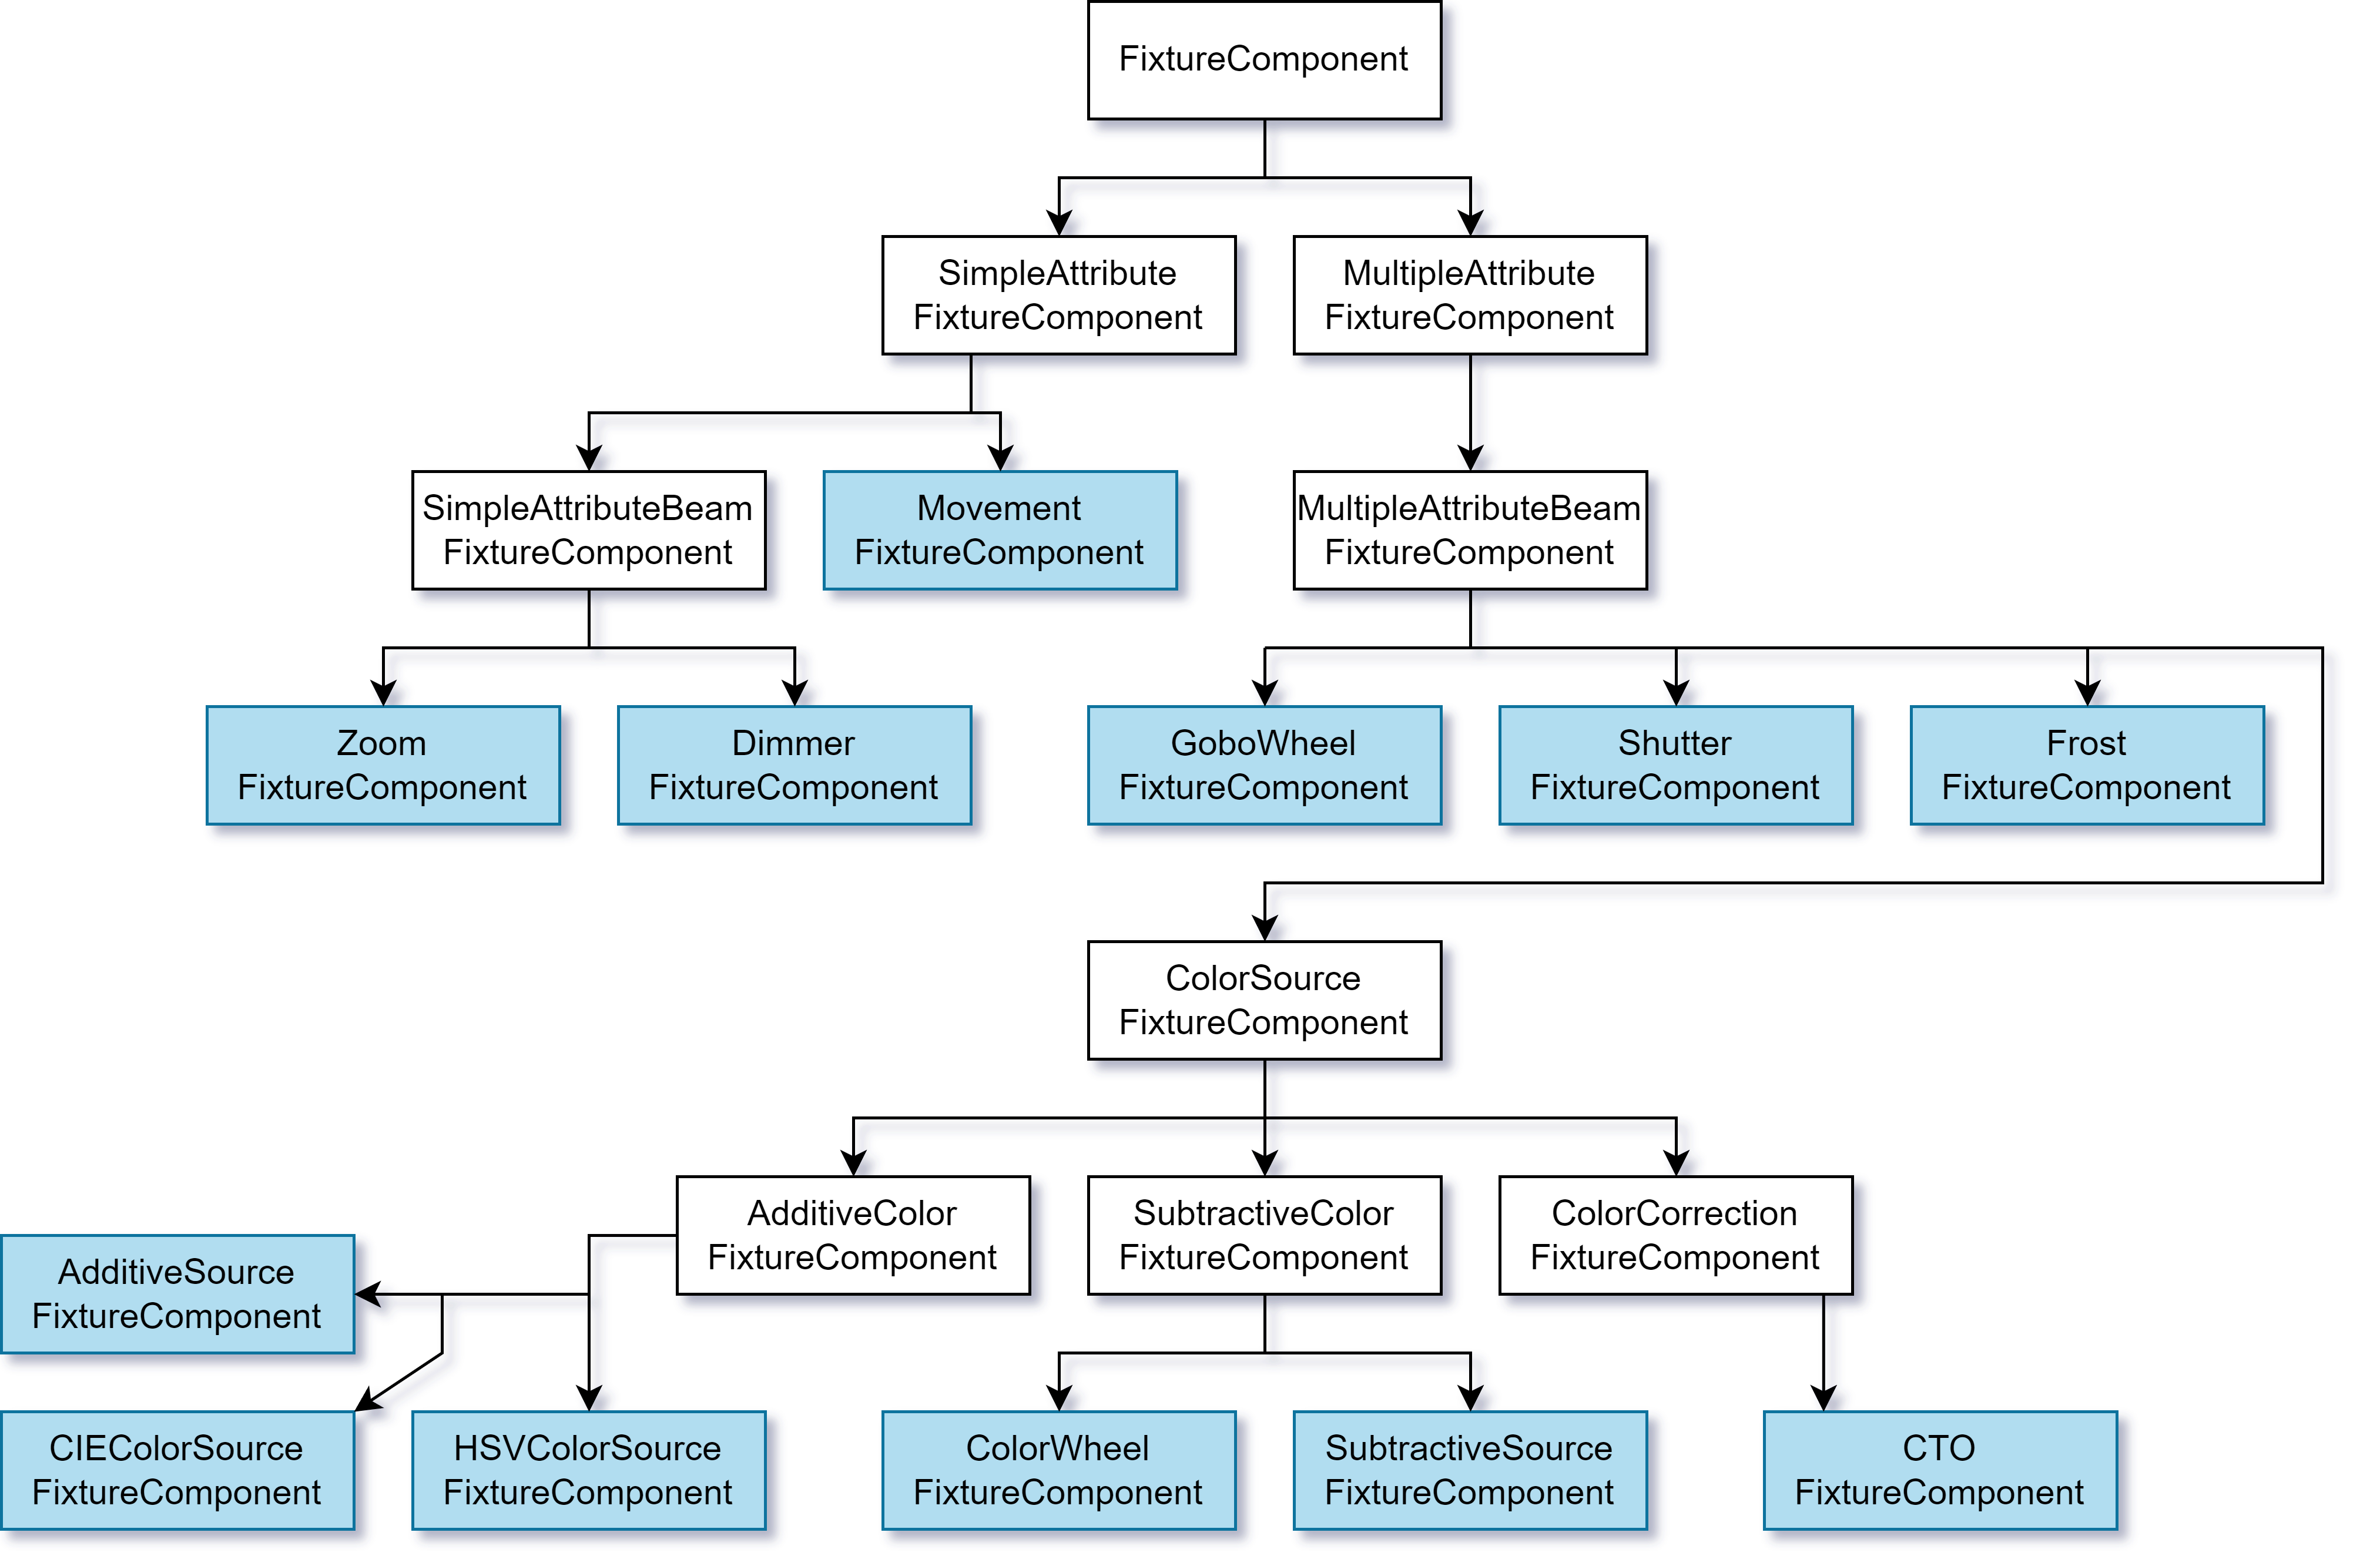
\includegraphics[width=0.9\linewidth]{img/fixtureComponent/FixtureComponentOLD.drawio.png}
    \caption{Struttura gerarchica delle classi FixtureComponent. In azzurro i componenti veri e propri.}
    \label{fig:3_fixtureComponentOld}
\end{figure}

\noindent I FixtureComponent vengono istanziati dalla classe \lstinline{FCPFActorComponentsLoader}, che si occupa anche di chiamare \lstinline{Setup()}. Setup è un metodo che viene essenzialmente duplicato in ogni componente e che si occupa di salvarsi il DMXChannel in cui il componente è presente, costruire un albero di LogicalChannel, salvarsi la geometria a cui si fa riferimento e ottenere il Canale DMX in cui è presente il componente. Quando una fixture istanziata in un mondo inizia ad essere emulata, viene chiamato \lstinline{BeginPlay()} su ogni suo componente che, attraverso del codice parzialmente duplicato, inizializzerà di nuovo l'albero dei LogicalChannel e inizializzerà l'interpolazione con dei valori hard-coded. A questo punto la fixture sarà \say{in esecuzione} e risponderà a due tipi di eventi:
\begin{itemize}
    \item \textbf{Nuovo pacchetto DMX}: Ogni volta che arriva un nuovo pacchetto DMX viene chiamata la funzione \lstinline{FixtureComponentBase::PushNormalizedRawValues()} che chiama a sua volta \lstinline{PushDMXRawValues()}. Quest'ultima funzione è implementata allo stesso identico modo su ogni singolo componente. Quello che fa è chiamare \lstinline{ApplyEffectToBeam()} con il valore dmx del canale. Se un componente riceve input da più DMXChannel, ci sarà una chiamata hard-coded per ciascuno, senza alcun ciclo che li scorra. \lstinline{ApplyEffectToBeam()} si occupa di interpretare i dati in arrivo. L'output di questo processo viene effettuato attraverso 3 funzioni: \lstinline{SetTargetValue()}, \lstinline{SetValueNoInterp()} e \lstinline{interp.SetValueNoInterp()}.
    \item \textbf{Viene eseguito un nuovo tick}: Viene chiamata \lstinline{InterpolateComponent()} che viene reimplementata da ogni componente ed in ciascuno si occupa di aggiornare lo stato interno degli effetti delle feature (esempio: FrostPulseOpen) controllate dallo stesso, utilizzando anche qui le funzioni \lstinline{SetTargetValue()}, \lstinline{SetValueNoInterp()} e \lstinline{interp.SetValueNoInterp()}. Successivamente aggiorna lo stato dell'interpolazione.
\end{itemize}
\lstinline{SetTargetValue()} è una funzione, attualmente reimplementata in maniera identica da tutti i componenti, che serve ad impostare un nuovo valore di destinazione all'interpolazione. Prima di impostare un nuovo target, controlla se l'interpolazione è attiva e se è già stato impostato un primo valore. In caso negativo, viene chiamata direttamente la funzione \lstinline{SetValueNoInterp()}, implementata dentro \lstinline{MultipleAttributeBeamFixtureComponent}, che si occupa di chiamare \lstinline{SetValueNoInterp_BeamInternal()} con un for su ogni geometria, che manda in output verso i materiali i valori elaborati dal componente.

\lstinline{interp.SetValueNoInterp()} è una funzione dell'oggetto interpolazione che lo fa saltare direttamente a quel valore.

\begin{figure}[H]
    \centering
    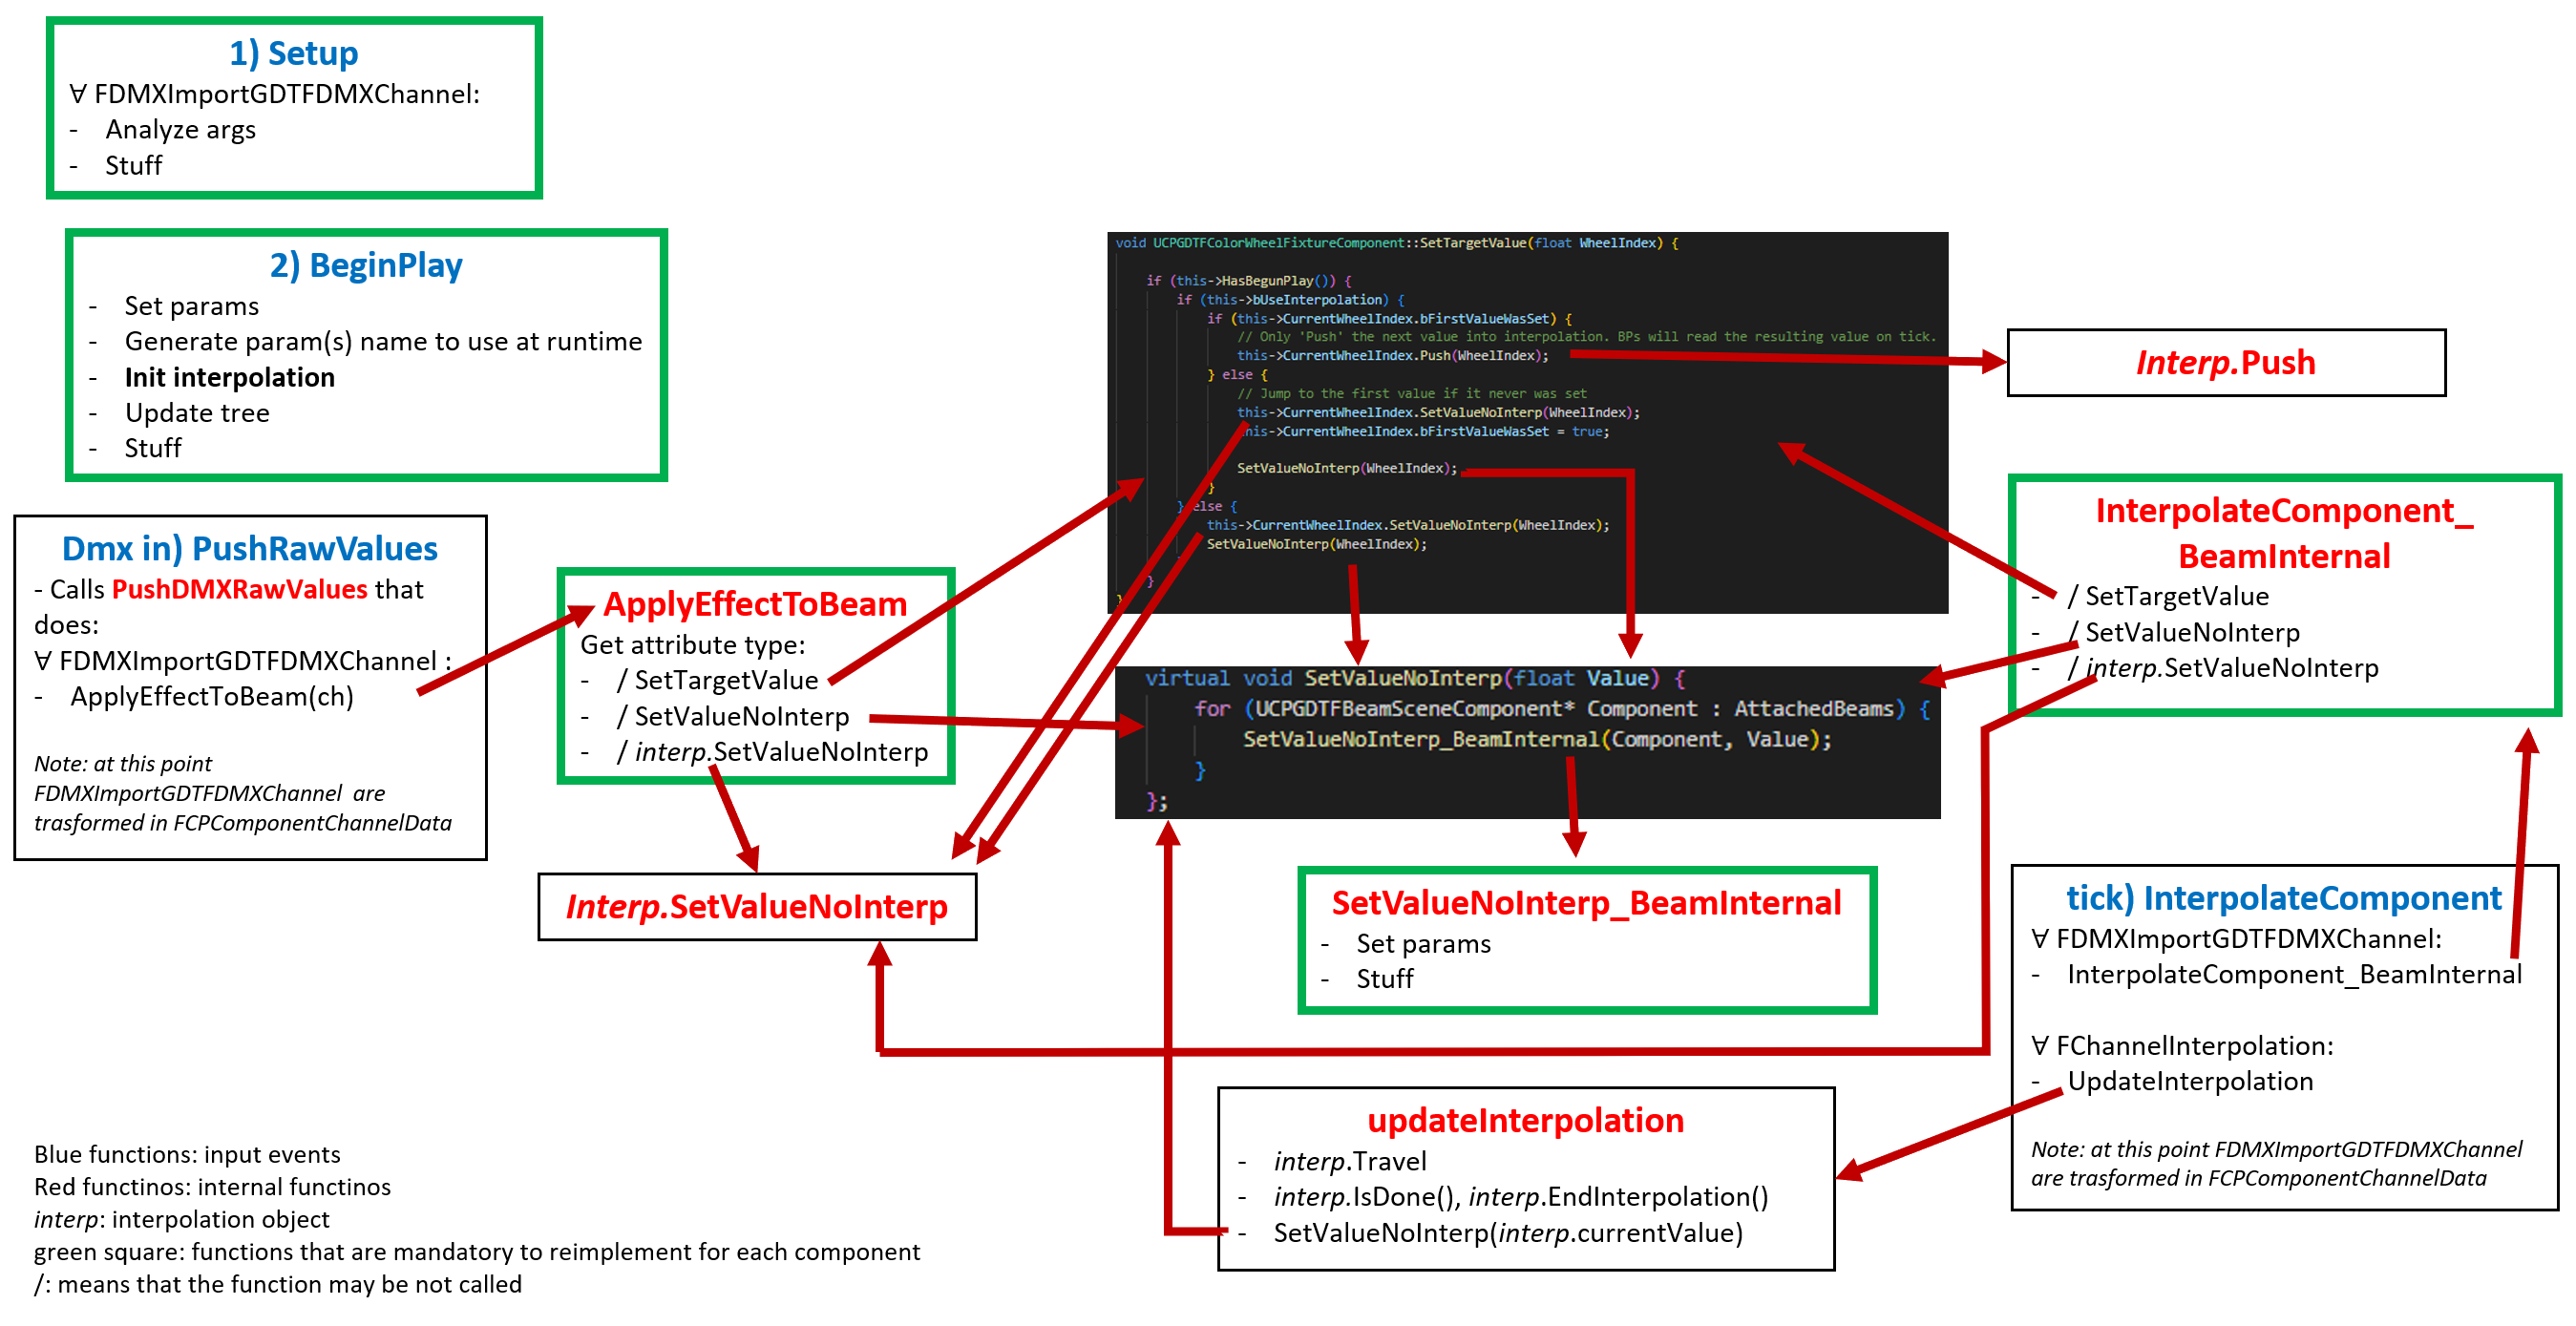
\includegraphics[width=1\linewidth]{img/fixtureComponent/CallOrderScheme.png}
    \caption{Schema creato in corso d'opera mentre svolgevo reverse-engineering sulla implementazione preesistente dei FixtureComponent. Le funzioni in azzurro sono triggerate da eventi esterni, quelle in rosso sono le funzioni interne. I quadrati verdi sono gli unici che, in una implementazione ideale, dovrebbero essere specializzati da ogni singolo componente.}
    \label{fig:3_CallOrderOld}
\end{figure}

\noindent Analizzando l'implementazione di questa gerarchia sono sorte delle criticità:
\begin{itemize}
    \item \textbf{Codice duplicato}: Nonostante alcune funzioni siano state dichiarate come virtuali in una classe padre, molte classi figlie le reimplementano in maniera identica l'una dall'altra. Un esempio è la funzione \lstinline{PushDMXRawValues()} che viene definita nello stesso identico modo da tutti i figli diretti di \lstinline{MultipleAttributeFixtureComponent}:
\lstset{language=UEcpp}
\begin{lstlisting}
void UCPGDTFFrostFixtureComponent::PushDMXRawValues(
        UDMXEntityFixturePatch* FixturePatch,
        const TMap<int32, int32>& RawValuesMap) {

	int32* DMXValuePtr = RawValuesMap.Find(this->ChannelAddress);
	if (DMXValuePtr) this->ApplyEffectToBeam(*DMXValuePtr);
}

void UCPGDTFShutterFixtureComponent::PushDMXRawValues(
        UDMXEntityFixturePatch* FixturePatch,
        const TMap<int32, int32>& RawValuesMap) {

	int32* DMXValuePtr = RawValuesMap.Find(this->ChannelAddress);
	if (DMXValuePtr) this->ApplyEffectToBeam(*DMXValuePtr);
}
\end{lstlisting}
    \item \textbf{Virtualizzazione delle funzioni quasi assente}: Molte funzioni sono presenti su vari componenti della gerarchia, ma non sono mai dichiarate su una classe padre, nonostante facciano la stessa cosa ed è giusto che siano esposte agli altri componenti. Un esempio sono \lstinline{ApplyEffectToBeam()} e \lstinline{SetTargetValue()} che sono implementate da molti componenti, ma mai definiti in un padre e sono anche un altro esempio di codice completamente duplicato.
    \item \textbf{Elementi superflui nella gerarchia}: Elementi come Simple o Multiple AttributeBeamFixtureComponent sono essenzialmente vuoti e non contribuiscono ad arricchire le sottoclassi, né ne aumentano la generalizzabilità.
    \item \textbf{Nessuna centralizzazione della gestione delle features}: La gerarchia viene definita attraverso delle classi che di fatto sono quasi delle interfacce. Questo comporta che la gestione di tutto che ci sta attorno ad una feature è a carico dei singoli componenti finali. Ogni volta che si implementa un nuovo componente si è quindi obbligati a reimplementare tutta la logica che sta dietro la gestione degli stessi.
    \item \textbf{Bassa chiarezza su cosa deve essere implementato nella singola feature}: Visti i punti precedenti, se si vuole implementare un nuovo componente senza avere conoscenze pregresse si rimane interdetti poiché non si capisce esattamente cosa bisogna fare. Non è presente una lista ben definita di funzionalità in cui il singolo componente deve specializzarsi.
    \item \textbf{Errori veri e propri nel calcolo di valori}: In generale, sono state riscontrate grosse mancanze con il calcolo di valori utili ad un componente. Ad esempio, il valore di minimo e massimo di una ChannelFunction viene calcolato solamente su quella corrente, piuttosto di avere un valore globale per tutti gli attributi dello stesso tipo. Oppure, i valori di fade e accelerazione per l'interpolazione non vengono proprio calcolati né presi dal GDTF originale.
    \item \textbf{Interpolazione mancante su molti componenti}: L'interpolazione non è gestita nella maniera corretta, di conseguenza è completamente mancante su molte feature di un faro, come ad esempio zoom, o rotazione di una gobo. Più specificatamente, è presente solamente sui componenti che estendono \lstinline{MultipleAttributesFixtureComponent} e se uno stesso componente controlla più features è attiva solo su una di esse.
    \item \textbf{Gestione di $N > 1$ canali hard-coded}: Se un componente gestisce più features oppure se riceve dati da più DMXChannel, la gestione di ogni singolo viene fatta copiando ed incollando il codice di uno più volte, piuttosto che avere dei for che li scorrono.
\end{itemize}

Per risolvere queste criticità è stato deciso un redesign dei vari FixtureComponent. A livello gerarchico non ci saranno molte differenze; esse saranno presenti maggiormente lato implementazione.

\subsection{Nuovo approccio}\label{subsec:3_idea}
Idealmente un componente dovrebbe definire pochi comportamenti specializzanti:
\begin{itemize}
    \item Costruttore del componente in cui, ad esempio, possono essere caricate eventuali texture o altre informazioni.
    \item \lstinline{BeginPlay()} per inizializzare i parametri dei Material e fornire i dati per inizializzare le interpolazioni.
    \item Definire gli AttributeGroups, ovvero una lista in cui vengono raggruppati attributi differenti del GDTF che però corrispondono alla stessa funzionalità (ES: \lstinline{Gobo_n_WheelShake} e \lstinline{Gobo_n_PosShake}) e che, a livello di scrittura di codice, vengono usati \say{insieme} dentro \lstinline{ApplyEffectToBeam()}. Attributi differenti che fanno parte dello stesso AttributeGroup condividono gli stessi valori default/min/max.
    \item Valori default per l'interpolazione, in caso non vengano forniti dal file GDTF.
    \item \lstinline{ApplyEffectToBeam()} per definire come una feature si deve comportare all'arrivo di nuovi valori DMX. Viene scorso a monte l'elenco dei canali per cui un componente è in ascolto e la funzione, a differenza di prima, deve ricevere tutte le informazioni del DMXChannel già elaborate, al posto di elaborarle da solo. 
    \item \lstinline{InterpolateComponent_BeamInternal()} per definire come la luce si deve comportare ad ogni tick, se ci sono effetti in esecuzione.
    \item \lstinline{SetValueNoInterp_BeamInternal()} per definire come inviare i dati elaborati dal componente verso il materiale. A differenza di prima questa funzione dovrà supportare più feature differenti, invece di avere un SetValueNoInterp specifico per ciascuna.
\end{itemize}

Tutto il resto invece dovrebbe essere appannaggio \say{automatico} dei padri, principalmente di \lstinline{FixtureComponentBase}. \newline

Nella nuova implementazione ogni FixtureComponent ha a disposizione 3 strutture dati principali: 
\begin{itemize}
    \item \lstinline{TArray<FCPComponentChannelData> channels}: Ogni \lstinline{FCPComponentChannelData} nell'array contiene informazioni su un particolare canale DMX fisico da cui il componente è dipendente, come il suo indirizzo ed il suo ultimo valore. All'interno di questa struttura sono stati spostati il DMXChannelTree e la variabile rappresentante l'attributo dell'ultima ChannelFunction che è stata eseguita. Per ogni pacchetto DMX che riceviamo, andiamo a chiamare \lstinline{ApplyEffectToBeam()} per ogni canale in questo array.
    \item \lstinline{TArray<FChannelInterpolation> interpolations}: Array contenente la lista di interpolazioni in esecuzione su questo determinato componente. Ogni interpolazione corrisponde a qualcosa che una vera luce muove fisicamente. Ciascuna ha un identificativo (chiamato \say{interpolationId}) corrispondente al suo indice nell'array, che viene spesso usato all'interno dei FixtureComponent per identificare a quale attributo esistente nella realtà ci stiamo riferendo. Un componente può avere $M$ canali ed $N$ componenti, non c'è una correlazione tra il numero dei due. Il target delle varie interpolazioni può essere impostato all'interno di \lstinline{ApplyEffectToBeam()} quando viene ricevuto un nuovo pacchetto DMX, oppure \lstinline{InterpolateComponent_BeamInternal()} ad ogni tick, specificando l'\lstinline{interpolationId} al quale vogliamo far riferimento. Inoltre, ad ogni tick, FixtureComponentBase scorrerà automaticamente tutto l'array di interpolazioni e ne aggiornerà lo stato.
    \item \lstinline{FAttributesData attributesData}: Struttura dati alla quale si possono fare delle query per ottenere dei \lstinline{FCPDMXChannelData}, ovvero i valori minimi, massimi, default, e di interpolazione, relativi ad un determinato attributo. Come già accennato precedentemente, attributi differenti che controllano una stessa identica feature possono essere raggruppati in dei set chiamati \say{AttributeGroup}. Poiché controllano la stessa feature, condivideranno anche gli stessi valori dentro \lstinline{attributesData}. Questa struttura dati viene usata anche per salvarsi la lista di AttributeGroup di un determinato FixtureComponent.
\end{itemize}

%\subsubsection{Strutture dati}\label{subsec:3_2_structs}

\subsection{Implementazione}\label{subsec:3_implementation}
Iniziamo con l'analizzare l'implementazione della struttura dati \lstinline{FAttributesData}. Tale struttura ha internamente memorizzata una lista di tutti i ChannelData presenti nel componente ed una mappa da attributo a ChannelData. Attributi che fanno parte dello stesso AttributeGroup verranno quindi risolti attraverso questa mappa, al medesimo ChannelData in memoria. \newline
\lstset{language=UEcpp}
%\begin{lstlisting}
%//Struttura dati che incapsula FCPDMXChannelData assieme
%//  all'attributeGroup di cui fa parte
%struct F__SingleAttributeData {
%    GENERATED_BODY()
%    UPROPERTY(VisibleDefaultsOnly, Category = "Internal")
%    TSet<ECPGDTFAttributeType> attributeGroup;
%    UPROPERTY(VisibleDefaultsOnly, Category = "Internal")
%    FCPDMXChannelData data;
%};
%
%UPROPERTY(VisibleDefaultsOnly, Category = "Internal")
%//Utilizziamo gli indici nella lista al posto di puntatori perche',
%//  altrimenti, UE non ne supporterebbe la serializzazione
%TMap<ECPGDTFAttributeType, int32> attributeData;
%UPROPERTY(VisibleDefaultsOnly, Category = "Internal")
%TArray<F__SingleAttributeData> attributeList;
%\end{lstlisting}
L'inserimento di un nuovo attributeGroup viene fatto aggiungendo prima uno \lstinline{F__SingleAttributeData} dentro la rispettiva lista e successivamente aggiungendo nella mappa ogni elemento del gruppo associato all'indice del precedente inserimento nella lista.\newline
La funzione \lstinline{FixtureComponentBase::Setup()} chiamerà due metodi: \lstinline{initAttributeGroups()} e \lstinline{analizeDMXChannels()}. Il primo dei due metodi si occupa di preallocare tutti gli attributeGroups con dei dati vuoti.
%\begin{lstlisting}
%void initAttributeGroups(
%        TArray<TSet<ECPGDTFAttributeType>> attributeGroups
%    ) {
%
%    attributeData.Empty();
%    attributeList.Empty();
%    for (int i = 0; i < attributeGroups.Num(); i++)
%        addAttributeData(attributeGroups[i]);
%}
%\end{lstlisting}
Il secondo invece si scorre ogni singola ChannelFunction presente dei DMXChannel in input e, per ciascuna, chiede alla \lstinline{FCPDMXChannelData} di aggiornare i propri valori. \newline
%\begin{lstlisting}
%void analizeDMXChannels(TArray<FDMXImportGDTFDMXChannel> DMXChannels) {
%    for (/*itera per ogni channelFunction cf dentro DMXChannels*/) {
%        ECPGDTFAttributeType attrType =
%            CPGDTFDescription::GetGDTFAttributeTypeValueFromString(
%                cf.Attribute.Name.ToString()
%            );
%        FCPDMXChannelData* channelData = getChannelData(attrType);
%        channelData->updateMinMaxFadeAccelCalc(cf);
%    }
%
%    for (int i = 0; i < attributeList.Num(); i++)
%        attributeList[i].data.finalizeMinMaxFadeAccelCalc();
%}
%\end{lstlisting}
Andiamo quindi a vedere come vengono calcolati i valori nella struttura dati \lstinline{FCPDMXChannelData}. Il problema principale da gestire è che spesso i valori di minimo e massimo di diversi attributi non sono indicati in ordine e per giunta, il valore minimo può non corrispondere al valore matematicamente più piccolo: Alcune funzionalità potrebbero essere invertite, quindi partire da un valore grande e finire ad uno piccolo. Tale caratteristica deve essere preservata ed automaticamente riconosciuta nel momento in cui si calcola un valore minimo e massimo globale per un attributeGroup. Inoltre, può capitare che attributi differenti dello stesso attributeGroup presentino valori differenti di fade e accelerazione anche se, da standard, dovrebbero essere uguali. La soluzione è fare la media tra i differenti valori, andando a gestire la casistica in cui in input abbiamo GDTF mal scritti. Per effettuare queste operazioni ci appoggiamo ad una struttura dati temporanea, che viene allocata automaticamente la prima volta che sopra viene chiamato \lstinline{updateMinMaxFadeAccelCalc()} e viene distrutta quando invece finalizziamo il calcolo:
\begin{lstlisting}
struct MinMaxHelper {
    //Numero di coppie from/to con from < to
    int normalNo = 0;
    //Numero di coppie from/to con from > to
    int invertedNo = 0;
    //Lista di tutti i valori from
    TArray<float> minArr;
    //Lista di tutti i valori to
    TArray<float> maxArr;

    //Somma di tutti i valori di fade ed accelerazione
    float fadeSum = 0, accelSum = 0;

    //Numero totale di elementi presenti
    float totalNo = 0;
    ~MinMaxHelper() {
        minArr.Empty();
        maxArr.Empty();
    }
};
MinMaxHelper* minMaxHelper = nullptr;
\end{lstlisting}
La funzione di update si occupa semplicemente di aggiungere i nuovi valori in input alle varie liste ed agli accumulatori. All'inizio controlla anche se l'attributo \lstinline{minMaxHelper} è nullo ed, in caso, lo alloca. Più interessante è invece la funzione che finalizza i calcoli. L'idea di base è ordinare i due array con i valori from ed i valori to in modo da ottenere i valori min/max assoluti, e decidere di prendere il primo o l'ultimo elemento da ciascuno in base a chi è più grande tra \lstinline{normalNo} e \lstinline{invertedNo}, controllando quindi se ci sono stati più coppie from/to \say{crescenti} che il contrario.
\begin{lstlisting}
void finalizeMinMaxFadeAccelCalc() {
    if (minMaxHelper == nullptr)
        return;
    
    minMaxHelper->minArr.Sort();
    minMaxHelper->maxArr.Sort();
    //Scegli quali valori usare
    bool isAsc = minMaxHelper->normalNo > minMaxHelper->invertedNo;
    //Ottieni i valori di massimo e minimo
    this->MaxValue = minMaxHelper->maxArr[
        isAsc  ? minMaxHelper->maxArr.Num() - 1 : 0;
    ];
    this->MinValue = minMaxHelper->minArr[
        !isAsc ? minMaxHelper->maxArr.Num() - 1 : 0;
    ];

    //Calcola i valori medi di fade e accelerazione
    float no = minMaxHelper->totalNo;
    interpolationFade = minMaxHelper->fadeSum / no;
    interpolationAcceleration = minMaxHelper->accelSum / no;

    //Elimina l'oggetto di helper
    delete minMaxHelper;
    minMaxHelper = nullptr;
}
\end{lstlisting}

A questo punto andiamo ad analizzare l'implementazione in se di una FixtureComponent.\newline

Come in precedenza, la vita di un FixtureComponent inizia con il metodo \lstinline{Setup()}, che creerà automaticamente un \lstinline{FCPComponentChannelData} per ogni canale DMX in input, per poi successivamente inizializzare la struttura dati \lstinline{FAttributesData attributesData}. Durante l'inizializzazione di quest'ultimo oggetto avverrà una chiamata a \lstinline{getAttributeGroups()} che dovrà essere definita dai componenti e restituirà una lista di set, ognuno rappresentante un attributeGroup. I componenti possono opzionalmente fare overriding del metodo \lstinline{Setup()} per effettuare operazioni extra in fase di caricamento come, ad esempio, caricare texture per le ruote.

Il metodo \lstinline{BeginPlay()} inizializzerà automaticamente le interpolazioni, creandone una per ogni AttributeGroup trovato all'interno di \lstinline{attributesData}. Anche questo metodo può subire overriding, in caso i componenti specifici vogliano inizializzare un numero di interpolazioni differente, oppure assegnargli diversi valori o un diverso ordine. Prima che venga inizializzata realmente l'interpolazione creando un nuovo oggetto \lstinline{FChannelInterpolation}, vengono generati i valori di fade e/o accelerazione se non erano già presenti nel GDTF originale. Ogni componente deve obbligatoriamente fare overriding di 2 metodi: \lstinline{float getDefaultRealAcceleration(int interpolationId)} e \lstinline{float getDefaultRealFade(int interpolationId)} che ci restituiscono un valore esatto in secondi di default, in caso nel GDTF manchi sia il valore di fade che quello di accelerazione. Se invece manca solamente uno dei due, l'altro viene ricalcolato automaticamente in base al rapporto tra fade ed accelerazione di default. Se a mancare è l'accelerazione, questa viene calcolata come:
\[accel = fade * \frac{defaultAccel}{defaultFade}\]
\clearpage %TODO CHECK IF THIS IS STILL NEEDED
Un po' più complicato invece è il calcolo del fade: durante il movimento una interpolazione accelera (in $accel$ secondi), rimane a velocità costante e poi decelera (di nuovo in $accel$ secondi). Il tempo di fade rappresenta la somma di tutti e tre questi momenti. Poiché già sappiamo quanto tempo impieghiamo ad accelerare e decelerare ($2 * accel$), ci interessa sapere quanto tempo rimaniamo a velocità costante rispetto a quanto tempo ci mettiamo ad accelerare. Quindi definiamo il tempo in cui rimaniamo a velocità costante come:
\[deafultConstantSpeedTime = deafaultFade - 2 * defaultAccel\] 
Ed il rapporto come:
\[defaultFadeRatio = \frac{deafultConstantSpeedTime}{defaultAccel} = \frac{deafaultFade - 2 * defaultAccel}{defaultAccel}\]
Per ottenere un valore di fade a partire da quello di accelerazione e dal defaultFadeRatio, basta invertire la formula:
\[fade = 2 * accel + accel * defaultFadeRatio\]

Nella nuova implementazione così come nella vecchia \lstinline{PushNormalizedRawValues()} chiama \lstinline{PushDMXRawValues()} ogni volta che arriva un nuovo pacchetto DMX. Nella nuova però \lstinline{PushDMXRawValues()} è implementato direttamente in \lstinline{FixtureComponentBase} e scorre automaticamente la lista di canali dmx del componente, invece di avere la lista hard-coded. Inoltre viene fatto un overloading della funzione \lstinline{ApplyEffectToBeam()}: \lstinline{PushDMXRawValues()} chiamerà prima una versione intermedia di questa funzione che si occuperà di ottenere e di passare già pre-calcolati il tipo dell'attributo ed il valore fisico del canale ad un'altra versione della stessa funzione, che dovrà essere implementata da ciascun componente. Questa operazione in precedenza era svolta e copia-incollata dentro ogni implementazione di \lstinline{ApplyEffectToBeam()} in tutti i componenti che estendevano \lstinline{FixtureComponentBase}.

\lstinline{SetTargetValue()}, precedentemente duplicata in ogni componente, è stata spostata nella logica di \lstinline{FixtureComponentBase}. Sia a \lstinline{SetTargetValue()} che a \lstinline{SetValueNoInterp()} è stato aggiunto in input l'id della interpolazione a cui vogliamo impostare il valore. 

Infine, viene modificata la funzione \lstinline{InterpolateComponent()}. Al posto di aggiornare in maniera hard-coded la lista di canali ed interpolazioni di un determinato componente, ora \lstinline{InterpolateComponent()} scorrerà prima la lista di canali e su ciascuno chiamerà \lstinline{InterpolateComponent_BeamInternal()} che dovrà essere implementata su ciascun componente e che si occuperà solamente di aggiornarne lo stato ad ogni tick. Poi, con un altro ciclo, aggiornerà tutte le varie interpolazioni, chiamando anche \lstinline{SetValueNoInterp()} con il valore di ciascuna.

\clearpage
\subsubsection{Ottenimento valori di default per le varie funzionalità di una fixture}\label{subsec:3_1_defaultValues}
Per l'ottenimento dei valori default dei vari componenti di una luce è stato purtroppo impossibile ottenere dati direttamente dalle fixture reali. Non esiste un modo attualmente implementato dalle fixture Claypaky per ottenere la posizione dei vari motori, anche se ci si collega direttamente in seriale alla scheda di controllo del faro. La soluzione adottata è stata quindi quella di filmare a rallentatore un faro ed inserire il video in un software di editing, in modo da contare con precisione il numero dei frame video che il faro impiega ad accelerare o decelerare ed il numero di frame che impiega a svolgere un movimento completo. Tramite questo metodo otteniamo una precisione pari a $\frac{1}{FPS}$, dove, sui telefoni moderni, FPS è uguale a 480 o addirittura 960.\newline

Successivamente è stata scritta una utility molto semplice in python per convertire automaticamente un numero espresso in \lstinline{secondi.frame} che ci viene dato direttamente dal programma di editing, in secondi nel mondo reale. \newline
Innanzitutto vengono specificato gli FPS del rallenty e gli FPS del video.
\lstset{language=python}
\begin{lstlisting}
SLOWMOTION_FPS = 480
VIDEO_FRAMERATE = 30
\end{lstlisting}
Poi dichiariamo una funzione che si occupa di convertire il numero di secondi che ci viene dato dal software di editing video in numero di frame totale, attraverso la formula:
\[totalFrames = secs * fps + frames\]
La usiamo quindi per convertire i valori in input:
\begin{lstlisting}
def convertFrames(s):
    sp = s.split(".")
    return int(sp[0]) * VIDEO_FRAMERATE + int(sp[1])

realFadeFrames = convertFrames(sys.argv[1])
realAccelFrames = convertFrames(sys.argv[2])
\end{lstlisting}

Infine ci calcoliamo quanti secondi dura un frame del video in slowmotion ed otteniamo i valori finali moltiplicando il numero di frame per la durata di ciascuno.
\begin{lstlisting}
#Calcoliamo quanto dura un frame
frameTime = 1 / SLOWMOTION_FPS

#Otteniamo il numero di secondi nel mondo reale
realFade = realFadeFrames * frameTime
realAccel = realAccelFrames * frameTime
\end{lstlisting}

\end{document}